%----------------------------------------------------------------------------------------
\begin{frame}
\begin{center}
\frametitle{Onion routing principles}
TODO: schema explicatif
\end{center}
\end{frame}


%---------------------------------------------------
\begin{frame}
\frametitle{TOR : The Onion Router}
It's an open-source implementation of the principles we just saw supported by
The Tor Project.
\begin{figure}

\includegraphics[width=0.5\linewidth]{./materials/septical_boy}
\end{figure}
\end{frame}
%---------------------------------------------------
\begin{frame}
\frametitle{TOR : The Onion Router}
\begin{block}{Pros}
\begin{itemize}
\item Hide you identity and location, prevents from eyesdropping.
\item Hide you browsing habbits and act like a debrider on the informations that
you're authorized to see.
\item encrypt your (incom|outgo)ing traffic between nodes.
\end{itemize}
\end{block}
\begin{block}{Cons}
\begin{itemize}
\item Slower connexion, forget about downloading big files, torrents
(deanonymize effect) etc...
\item Still vulnerable to some kind of analysis
\\ (timing deduction or infection between applications).
\item entry/exit nodes are vulnerables, no magic here.
\\ (Partial solution if you setup an exit enclaving node)
\end{itemize}
\end{block}
TOR is an anonymity tool, not a security one.
\end{frame}

%---------------------------------------------------
\begin{frame}
\frametitle{If you use it, do it smartly}
\begin{columns}[c]
\column{.5\textwidth}
\begin{itemize}
\item don't use standalone TOR or Vidalia bundlle
\item prefer the use of the TBB (Tor Browser Bundle)
\item or even better : tails (live Debian), in hostile environment
(public places etc)
\end{itemize}
\column{.5\textwidth}
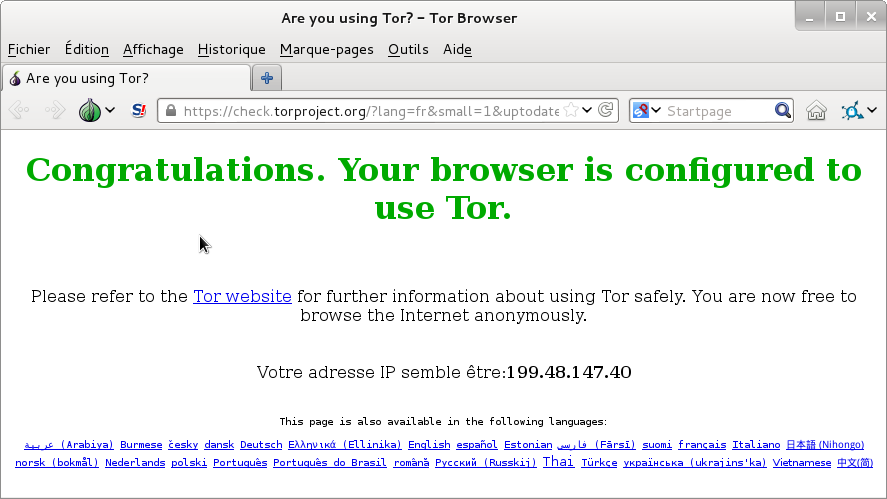
\includegraphics[keepaspectratio,width=\textwidth, height=.8\textheight]{./materials/tbb}
\end{columns}
Try Tor browser launcher for your distribution, that keep TBB updated. Grab-it
from here :\\ https://github.com/micahflee/torbrowser-launcher
\end{frame}
%----------------------------------------------------------------------------------------
\begin{frame}
\begin{center}
\Huge{If it's free, then you're the product}
\end{center}
\end{frame}

%----------------------------------------------------------------------------------------
\begin{frame}
\frametitle{What is the tracking ?}

\begin{block}{Tracking over the Internet}
\begin{itemize}
\justifying{
\item websites, announcers use it to learn your browsing habbits.
\item they save what website are you visiting, what do you like or not and
what you buy.
\item Data are processed in order to display the best ads that fit your
preferences.
}
\end{itemize}
\end{block}
\end{frame}


%----------------------------------------------------------------------------------------
\begin{frame}
\frametitle{What's the magic ?}

\justifying{
\begin{block}{Ads and widget are spying you}
\begin{itemize}
\item The Like button : allows FaceBook to know what you visit, even if you
don't click on it, even if you are properly disconnected from Facebook.
\item Same for the +1 by Google, and Google Analytics script.
\item In fact every ads and many widget do it.
\end{itemize}
\end{block}
}
\begin{center}

\includegraphics[scale=0.3] {./materials/Facebook_like.png}
\end{center}
\end{frame}

%----------------------------------------------------------------------------------------
\begin{frame}
\frametitle{Want to test ? Try LightBeam (ex Collusion) with Firefox}
That add-on allow you to see in real time which websites are tracking you
and the inter-connexion between the actual website and others. Kind of weird
sometime.
\begin{center}
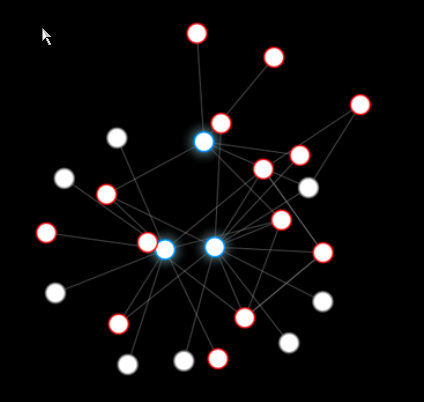
\includegraphics[scale=0.3] {./materials/Collusion.png}
\end{center}
\end{frame}

%----------------------------------------------------------------------------------------
\begin{frame}
\begin{center}
\Huge{Anomymat et extensions pour Firefox}
\end{center}
\end{frame}


%----------------------------------------------------------------------------------------
\begin{frame}
\frametitle{Noscript}

Bloque tous les trackers associés au site.

\begin{center}

\end{center}
\end{frame}


%----------------------------------------------------------------------------------------
\begin{frame}
\frametitle{Self destructing cookie}

Suppression automatisée des cookies

\begin{center}
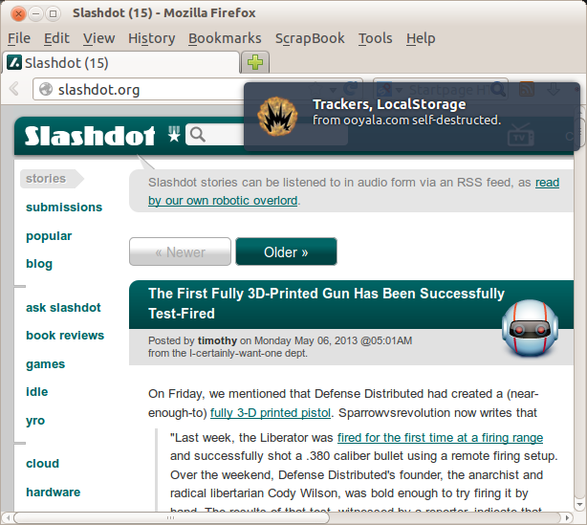
\includegraphics[scale=0.4] {./materials/selfdestructingcookie.png}
\end{center}
\end{frame}

%----------------------------------------------------------------------------------------
\begin{frame}
\begin{center}
\Huge{Changer de moteur de recherche}
\end{center}
\end{frame}

%----------------------------------------------------------------------------------------
\begin{frame}
\begin{center}
\frametitle{Duckduckgo - Google tracks you. We don't.}

\url{https://duckduckgo.com/}
\\

\includegraphics[scale=0.4] {./materials/DuckDuckGo.jpg}
\end{center}
\end{frame}

%----------------------------------------------------------------------------------------
\begin{frame}
\begin{center}
\Huge{Et pour plus de sécurité?}
\end{center}
\end{frame}

%----------------------------------------------------------------------------------------
\begin{frame}
\frametitle{HTTPSEverywhere}

Force le passage en https quand celui-ci est proposé par le site.

\begin{center}

\includegraphics[scale=0.4] {./materials/https-everywhere.jpg}
\end{center}

\end{frame}

%----------------------------------------------------------------------------------------
\begin{frame}
\frametitle{Certificate Patrol}
Permet de valider les certificats d'un site (lié à https).
\begin{center}
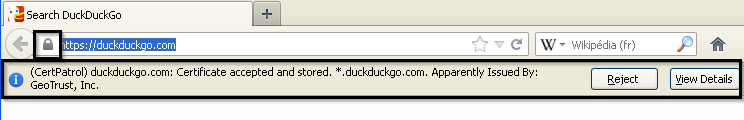
\includegraphics[scale=0.4] {./materials/CertificatePatrol.png}
\end{center}
\end{frame}

